%% Time-stamp: <2019-01-22 14:47:04 (marc)>
\documentclass[xcolor=x11names,compress,mathserif]{beamer}

\usepackage{../includes/MarkMathCmds}


\newcommand{\hackspace}{\hspace{4.2mm}}
\newcommand{\showstudent}[1]{}



% talk/author information
\newcommand{\authorname}{Mark van der Wilk}
\newcommand{\authoremail}{m.vdwilk@imperial.ac.uk}
\newcommand{\authoraffiliation}{
 Department of Computing\\Imperial
  College London}
\newcommand{\authortwitter}{markvanderwilk}
\newcommand{\slidesettitle}{\imperialBlue{Reasoning with Uncertainty}}
\newcommand{\footertitle}{Reasoning with Uncertainty}
\newcommand{\location}{Imperial College London}
\newcommand{\talkDate}{{January 16, 2023}}

\usepackage{subfig}




\date{\imperialGray{\talkDate}}




% load defaults
\selectcolormodel{rgb}
\usepackage{ifxetex,ifluatex}
\newif\ifxetexorluatex
\ifxetex
  \xetexorluatextrue
\else
  \ifluatex
    \xetexorluatextrue
  \else
    \xetexorluatexfalse
  \fi
\fi

\usepackage{textpos}
%\usepackage{arabtex}
\usepackage{tikz}
\usetikzlibrary{decorations.markings}
\usetikzlibrary{arrows}
\usetikzlibrary{shapes}
\usetikzlibrary{plotmarks}
\usetikzlibrary{mindmap,trees,backgrounds}

\tikzstyle{every picture}+=[remember picture]

%\usepackage{movie15}
% \usepackage{pdfpages}
%\usepackage{xmpmulti}

\usepackage{anyfontsize}
\usepackage{wrapfig}
\usepackage{animate}
\usepackage{multirow}
\usepackage{multimedia}
\usepackage{xmpmulti}
%\usepackage[latin9]{inputenc}
\usepackage[english]{babel}
\usepackage{scalefnt}
\usepackage{verbatim}
\usepackage{url}
% \usepackage{pgf,pgfarrows,pgfnodes}
\usepackage{textpos}
\usepackage[tight,ugly]{units}
\usepackage{url}
\usepackage{bbm}
\usepackage[english]{babel}
\usepackage{fancyhdr}
\usepackage{bm} % correct bold symbols, like \bm
\usepackage{amsmath}
\usepackage{amsfonts}
\usepackage{amssymb}
\usepackage{mathrsfs}
\usepackage{mathtools}
\usepackage{color}
\usepackage{cancel}
\usepackage{algorithm}
\usepackage{algpseudocode}
\usepackage{mathrsfs}
\usepackage{listings}
\usepackage{graphicx} % for pdf, bitmapped graphics files
\usepackage{mathtools}
\usepackage{units}
\usepackage{subfig}
\usepackage{enumerate}
\usepackage{natbib}
\usepackage{dsfont}


\ifxetexorluatex
\usepackage{fontspec}
\setmainfont[Scale=0.8]{OpenDyslexic-Regular}
\else
\usefonttheme{professionalfonts}
\fi

\renewcommand{\vec}[1]{{\boldsymbol{{#1}}}} % vector
\newcommand{\mat}[1]{{\boldsymbol{{#1}}}} % matrix
% \newcommand{\KL}[2]{\mathrm{KL}(#1\|#2)} % KL divergence
\newcommand{\R}[0]{\mathds{R}} % real numbers
\newcommand{\Z}[0]{\mathds{Z}} % integers
\newcommand{\tr}[0]{\text{tr}} % trace
% \newcommand{\inv}{^{-1}}
% \DeclareMathOperator*{\diag}{diag}
\newcommand{\E}{\mathds{E}} % expectation
\newcommand{\var}{\mathds{V}}
\newcommand{\gauss}[2]{\mathcal{N}\big(#1,\,#2\big)}
\newcommand{\gaussx}[3]{\mathcal{N}\big(#1\,|\,#2,\,#3\big)}
\newcommand{\gaussBig}[2]{\mathcal{N}\left(#1,\,#2\right)}
\newcommand{\gaussxBig}[3]{\mathcal{N}\left(#1\,\left|\,#2,\,#3\right.\right)}
\newcommand{\Ber}[0]{\mathrm{Ber}} % Bernoulli distribution
\DeclareMathOperator{\cov}{Cov}
\ifxetexorluatex
\renewcommand{\T}[0]{^\top}
\renewcommand{\d}[0]{\text{d}} % derivative
\else
\newcommand{\T}[0]{^\top}
\renewcommand{\d}[0]{\text{d}} % derivative
\fi
% calculus
\newcommand{\pdiff}[1]{\frac{\partial}{\partial #1}}
\newcommand{\pdiffF}[2]{\frac{\partial #1}{\partial #2}}
\newcommand{\diffF}[2]{\frac{{\d}#1}{{\d}#2}}
\newcommand{\diffFII}[2]{\frac{{\d}^2 #1}{{\d}#2^2}}
\newcommand{\diff}[1]{\frac{{\d}}{{\d}#1}}
\newcommand{\diffII}[1]{\frac{{\d}^2}{{\d}#1^2}}
\newcommand{\class}[0]{\mathcal{C}}

\newcommand{\idx}[1]{^{(#1)}}
% \newcommand{\norm}[1]{\left\|#1\right\|}
\newcommand{\proj}[1]{\tilde{#1}}
\newcommand{\pcacoord}{z}
\newcommand{\pcacoordnew}{\zeta}
\newcommand{\latent}{z}
% \newcommand{\given}{\,|\,}
\newcommand{\genset}[1]{\mathrm{span}[#1]} % generating set
\newcommand{\set}[1]{\mathcal{#1}} % set
\newcommand{\fixgmfont}[1]{\scalebox{0.8}{#1}}



\usepackage{pifont}% http://ctan.org/pkg/pifont
\newcommand{\cmark}{{\color{green!40!black}\ding{51}}}%
\newcommand{\xmark}{{\color{red}\ding{55}}}%
\newcommand{\green}[1]{{\bf{\textcolor{green}{#1}}}}
\newcommand{\red}[1]{{\bf{\textcolor{red}{#1}}}}

\newcommand<>\red[1]{{\color#2[rgb]{1,0,0}#1}}
\newcommand<>\blue[1]{{\color#2[rgb]{0,0,1}#1}}
\newcommand<>\yellow[1]{{\color#2{camyellow}#1}}
\newcommand<>\green[1]{{\color#2[rgb]{0,0.6,0.0}#1}}
\newcommand<>\violet[1]{{\color#2[rgb]{0.6,0,0.6}#1}}
\newcommand<>\orange[1]{{\color#2[rgb]{1,0.5,0}#1}}
\newcommand<>\black[1]{{\color#2[rgb]{0,0,0}#1}}
\newcommand<>\steel[1]{{\color#2[rgb]{0,0,0.8}#1}}
\newcommand<>\darkblue[1]{{\color#2[rgb]{0,0,0.6}#1}}
\newcommand<>\lightblue[1]{{\color#2[rgb]{0.4,0.4,0.7}#1}}
\newcommand<>\gray[1]{{\color#2[rgb]{0.4,0.4,0.4}#1}}
\newcommand<>\greenish[1]{{\color#2[rgb]{0.45, 0.66, 0.45}#1}}
\newcommand<>\redish[1]{{\color#2[rgb]{0.7843    0.3706    0.3706}#1}}
\definecolor{redishTIKZ}{rgb}{0.7843, 0.3706, 0.3706}
\definecolor{imperialBlue}{rgb}{0.058, 0.219, 0.418}
\definecolor{aimsbrown}{rgb}{0.539, 0.117, 0.015}
% \definecolor{imperialGray}{rgb}{0.414, 0.488, 0.671 }
\definecolor{imperialGray}{RGB}{109,153, 204}
\definecolor{aimslightbrown}{RGB}{138,88,84}
\newcommand<>\imperialBlue[1]{{\color#2[rgb]{0.058, 0.219, 0.418}#1}}
\newcommand<>\aimsbrown[1]{{\color#2[rgb]{0.539, 0.117, 0.015}#1}}
%\newcommand<>\imperialGray[1]{{\color#2[rgb]{0.414, 0.488, 0.671}#1}}
\newcommand<>\imperialGray[1]{{\color#2[RGB]{109,153, 204}#1}}
\newcommand<>\aimslightbrown[1]{{\color#2[RGB]{138,88,84}#1}}
\newcommand<>\lightgray[1]{{\color#2[rgb]{0.8,0.8,0.8}#1}}
%\newcommand<>\highlightcolor[1]{{\color#2[rgb]{0,0,1}#1}}
\newcommand{\highlight}[1]{{\bf\steel{#1}}}
%\newcommand{\newblock}[0]{}

%\newcommand{\arrow}[0]{\includegraphics[height=5pt]{./figures/arrow}\hspace{3pt}}

\renewcommand{\emph}[1]{\textbf{\steel{{#1}}}}

\renewcommand{\alert}[1]{{\bf\red{{#1}}}}

\newcommand{\arrow}{
\begin{tikzpicture}
\draw [black!40!green, fill=black!40!green] (0,-0.12) -- (0,0.12) --
(0.15,0);
\draw [black!40!green, fill=black!40!green] (0.15,-0.12) -- (0.15,0.12) --
(0.3,0); 
\end{tikzpicture}
}

\geometry{left=0.45cm,top=0cm,right=0.45cm}


\newcommand{\logoimagepath}{./figures/imperial}
\newcommand{\highlightcolor}{blue!80!black}
%\newcommand{\headbarcolor}{imperialBlue}
\newcommand{\headbarcolor}{imperialBlue}
\institute{}

\newcommand{\coursetitle}{}

\newcommand{\slidesetsubtitle}{}
\newcommand{\slidesetnumber}{01}
\usefonttheme{professionalfonts}


\usetikzlibrary{decorations.fractals}
% tikzlibrary.code.tex
%
% Copyright 2010-2011 by Laura Dietz
% Copyright 2012 by Jaakko Luttinen
%
% The MIT License
%
% See LICENSE file for more details.

% Load other libraries
\usetikzlibrary{shapes}
\usetikzlibrary{fit}
\usetikzlibrary{chains}
\usetikzlibrary{arrows}

% Latent node
\tikzstyle{latent} = [circle,fill=white,draw=black,inner sep=1pt,
minimum size=20pt, font=\fontsize{10}{10}\selectfont, node distance=1]
% Observed node
\tikzstyle{obs} = [latent,fill=gray!25]
% Constant node
\tikzstyle{const} = [rectangle, inner sep=0pt, node distance=1]
% Factor node
\tikzstyle{factor} = [rectangle, fill=black,minimum size=5pt, inner
sep=0pt, node distance=0.4]
% Deterministic node
\tikzstyle{det} = [latent, diamond]

% Plate node
\tikzstyle{plate} = [draw, rectangle, rounded corners, fit=#1]
% Invisible wrapper node
\tikzstyle{wrap} = [inner sep=0pt, fit=#1]
% Gate
\tikzstyle{gate} = [draw, rectangle, dashed, fit=#1]

% Caption node
\tikzstyle{caption} = [font=\footnotesize, node distance=0] %
\tikzstyle{plate caption} = [caption, node distance=0, inner sep=0pt,
below left=5pt and 0pt of #1.south east] %
\tikzstyle{factor caption} = [caption] %
\tikzstyle{every label} += [caption] %

%\pgfdeclarelayer{b}
%\pgfdeclarelayer{f}
%\pgfsetlayers{b,main,f}

% \factoredge [options] {inputs} {factors} {outputs}
\newcommand{\factoredge}[4][]{ %
  % Connect all nodes #2 to all nodes #4 via all factors #3.
  \foreach \f in {#3} { %
    \foreach \x in {#2} { %
      \path (\x) edge[-,#1] (\f) ; %
      %\draw[-,#1] (\x) edge[-] (\f) ; %
    } ;
    \foreach \y in {#4} { %
      \path (\f) edge[->, >={triangle 45}, #1] (\y) ; %
      %\draw[->,#1] (\f) -- (\y) ; %
    } ;
  } ;
}

% \edge [options] {inputs} {outputs}
\newcommand{\edge}[3][]{ %
  % Connect all nodes #2 to all nodes #3.
  \foreach \x in {#2} { %
    \foreach \y in {#3} { %
      \path (\x) edge [->, >={triangle 45}, #1] (\y) ;%
      %\draw[->,#1] (\x) -- (\y) ;%
    } ;
  } ;
}

% \factor [options] {name} {caption} {inputs} {outputs}
\newcommand{\factor}[5][]{ %
  % Draw the factor node. Use alias to allow empty names.
  \node[factor, label={[name=#2-caption]#3}, name=#2, #1,
  alias=#2-alias] {} ; %
  % Connect all inputs to outputs via this factor
  \factoredge {#4} {#2-alias} {#5} ; %
}

% \plate [options] {name} {fitlist} {caption}
\newcommand{\plate}[4][]{ %
  \node[wrap=#3] (#2-wrap) {}; %
  \node[plate caption=#2-wrap] (#2-caption) {#4}; %
  \node[plate=(#2-wrap)(#2-caption), #1] (#2) {}; %
}

% \gate [options] {name} {fitlist} {inputs}
\newcommand{\gate}[4][]{ %
  \node[gate=#3, name=#2, #1, alias=#2-alias] {}; %
  \foreach \x in {#4} { %
    \draw [-*,thick] (\x) -- (#2-alias); %
  } ;%
}

% \vgate {name} {fitlist-left} {caption-left} {fitlist-right}
% {caption-right} {inputs}
\newcommand{\vgate}[6]{ %
  % Wrap the left and right parts
  \node[wrap=#2] (#1-left) {}; %
  \node[wrap=#4] (#1-right) {}; %
  % Draw the gate
  \node[gate=(#1-left)(#1-right)] (#1) {}; %
  % Add captions
  \node[caption, below left=of #1.north ] (#1-left-caption)
  {#3}; %
  \node[caption, below right=of #1.north ] (#1-right-caption)
  {#5}; %
  % Draw middle separation
  \draw [-, dashed] (#1.north) -- (#1.south); %
  % Draw inputs
  \foreach \x in {#6} { %
    \draw [-*,thick] (\x) -- (#1); %
  } ;%
}

% \hgate {name} {fitlist-top} {caption-top} {fitlist-bottom}
% {caption-bottom} {inputs}
\newcommand{\hgate}[6]{ %
  % Wrap the left and right parts
  \node[wrap=#2] (#1-top) {}; %
  \node[wrap=#4] (#1-bottom) {}; %
  % Draw the gate
  \node[gate=(#1-top)(#1-bottom)] (#1) {}; %
  % Add captions
  \node[caption, above right=of #1.west ] (#1-top-caption)
  {#3}; %
  \node[caption, below right=of #1.west ] (#1-bottom-caption)
  {#5}; %
  % Draw middle separation
  \draw [-, dashed] (#1.west) -- (#1.east); %
  % Draw inputs
  \foreach \x in {#6} { %
    \draw [-*,thick] (\x) -- (#1); %
  } ;%
}


% Copyright (C) 2016  Joseph Rabinoff

% ipe2tikz is free software; you can redistribute it and/or modify it under
% the terms of the GNU General Public License as published by the Free
% Software Foundation; either version 3 of the License, or (at your option)
% any later version.

% ipe2tikz is distributed in the hope that it will be useful, but WITHOUT ANY
% WARRANTY; without even the implied warranty of MERCHANTABILITY or FITNESS
% FOR A PARTICULAR PURPOSE.  See the GNU General Public License for more
% details.

% You should have received a copy of the GNU General Public License along with
% ipe2tikz; if not, you can find it at "http://www.gnu.org/copyleft/gpl.html",
% or write to the Free Software Foundation, Inc., 675 Mass Ave, Cambridge, MA
% 02139, USA.


% ipe compatibility TikZ styles

\usetikzlibrary{arrows.meta}

\makeatletter

% These should behave almost exactly like ipe arrows.  They disable correcting
% for the miter length and line width.  This is important for visual consistency
% with ipe, since ipe arrows get much larger when the line width is increased.
% They also use the line join and cap styles from the main path.  These are very
% simple arrows: there is no harpoon version, and the convex hull computation is
% sloppy.

\pgfdeclarearrow{
  name = ipe _linear,
  defaults = {
    length = +1bp,
    width  = +.666bp,
    line width = +0pt 1,
  },
  setup code = {
    % Control points
    \pgfarrowssetbackend{0pt}
    \pgfarrowssetvisualbackend{
      \pgfarrowlength\advance\pgf@x by-.5\pgfarrowlinewidth}
    \pgfarrowssetlineend{\pgfarrowlength}
    \ifpgfarrowreversed
      \pgfarrowssetlineend{\pgfarrowlength\advance\pgf@x by-.5\pgfarrowlinewidth}
    \fi
    \pgfarrowssettipend{\pgfarrowlength}
    % Convex hull
    \pgfarrowshullpoint{\pgfarrowlength}{0pt}
    \pgfarrowsupperhullpoint{0pt}{.5\pgfarrowwidth}
    % The following are needed in the code:
    \pgfarrowssavethe\pgfarrowlinewidth
    \pgfarrowssavethe\pgfarrowlength
    \pgfarrowssavethe\pgfarrowwidth
  },
  drawing code = {
    \pgfsetdash{}{+0pt}
    \ifdim\pgfarrowlinewidth=\pgflinewidth\else\pgfsetlinewidth{+\pgfarrowlinewidth}\fi
    \pgfpathmoveto{\pgfqpoint{0pt}{.5\pgfarrowwidth}}
    \pgfpathlineto{\pgfqpoint{\pgfarrowlength}{0pt}}
    \pgfpathlineto{\pgfqpoint{0pt}{-.5\pgfarrowwidth}}
    \pgfusepathqstroke
  },
  parameters = {
    \the\pgfarrowlinewidth,%
    \the\pgfarrowlength,%
    \the\pgfarrowwidth,%
  },
}


\pgfdeclarearrow{
  name = ipe _pointed,
  defaults = {
    length = +1bp,
    width  = +.666bp,
    inset  = +.2bp,
    line width = +0pt 1,
  },
  setup code = {
    % Control points
    \pgfarrowssetbackend{0pt}
    \pgfarrowssetvisualbackend{\pgfarrowinset}
    \pgfarrowssetlineend{\pgfarrowinset}
    \ifpgfarrowreversed
      \pgfarrowssetlineend{\pgfarrowlength}
    \fi
    \pgfarrowssettipend{\pgfarrowlength}
    % Convex hull
    \pgfarrowshullpoint{\pgfarrowlength}{0pt}
    \pgfarrowsupperhullpoint{0pt}{.5\pgfarrowwidth}
    \pgfarrowshullpoint{\pgfarrowinset}{0pt}
    % The following are needed in the code:
    \pgfarrowssavethe\pgfarrowinset
    \pgfarrowssavethe\pgfarrowlinewidth
    \pgfarrowssavethe\pgfarrowlength
    \pgfarrowssavethe\pgfarrowwidth
  },
  drawing code = {
    \pgfsetdash{}{+0pt}
    \ifdim\pgfarrowlinewidth=\pgflinewidth\else\pgfsetlinewidth{+\pgfarrowlinewidth}\fi
    \pgfpathmoveto{\pgfqpoint{\pgfarrowlength}{0pt}}
    \pgfpathlineto{\pgfqpoint{0pt}{.5\pgfarrowwidth}}
    \pgfpathlineto{\pgfqpoint{\pgfarrowinset}{0pt}}
    \pgfpathlineto{\pgfqpoint{0pt}{-.5\pgfarrowwidth}}
    \pgfpathclose
    \ifpgfarrowopen
      \pgfusepathqstroke
    \else
      \ifdim\pgfarrowlinewidth>0pt\pgfusepathqfillstroke\else\pgfusepathqfill\fi
    \fi
  },
  parameters = {
    \the\pgfarrowlinewidth,%
    \the\pgfarrowlength,%
    \the\pgfarrowwidth,%
    \the\pgfarrowinset,%
    \ifpgfarrowopen o\fi%
  },
}


% For correcting minipage width in stretched nodes
\newdimen\ipeminipagewidth
\def\ipestretchwidth#1{%
  \pgfmathsetlength{\ipeminipagewidth}{#1/\ipenodestretch}}

\tikzstyle{ipe import} = [
  % General ipe defaults
  x=1bp, y=1bp,
%
  % Nodes
  ipe node stretch/.store in=\ipenodestretch,
  ipe stretch normal/.style={ipe node stretch=1},
  ipe stretch normal,
  ipe node/.style={
    anchor=base west, inner sep=0, outer sep=0, scale=\ipenodestretch
  },
%
  % Use a special key for the mark scale, so that the default can be overriden.
  % (This doesn't happen with the scale= key; those accumulate.)
  ipe mark scale/.store in=\ipemarkscale,
%
  ipe mark tiny/.style={ipe mark scale=1.1},
  ipe mark small/.style={ipe mark scale=2},
  ipe mark normal/.style={ipe mark scale=3},
  ipe mark large/.style={ipe mark scale=5},
%
  ipe mark normal, % Set default
%
  ipe circle/.pic={
    \draw[line width=0.2*\ipemarkscale]
      (0,0) circle[radius=0.5*\ipemarkscale];
    \coordinate () at (0,0);
  },
  ipe disk/.pic={
    \fill (0,0) circle[radius=0.6*\ipemarkscale];
    \coordinate () at (0,0);
  },
  ipe fdisk/.pic={
    \filldraw[line width=0.2*\ipemarkscale]
      (0,0) circle[radius=0.5*\ipemarkscale];
    \coordinate () at (0,0);
  },
  ipe box/.pic={
    \draw[line width=0.2*\ipemarkscale, line join=miter]
      (-.5*\ipemarkscale,-.5*\ipemarkscale) rectangle
      ( .5*\ipemarkscale, .5*\ipemarkscale);
    \coordinate () at (0,0);
  },
  ipe square/.pic={
    \fill
      (-.6*\ipemarkscale,-.6*\ipemarkscale) rectangle
      ( .6*\ipemarkscale, .6*\ipemarkscale);
    \coordinate () at (0,0);
  },
  ipe fsquare/.pic={
    \filldraw[line width=0.2*\ipemarkscale, line join=miter]
      (-.5*\ipemarkscale,-.5*\ipemarkscale) rectangle
      ( .5*\ipemarkscale, .5*\ipemarkscale);
    \coordinate () at (0,0);
  },
  ipe cross/.pic={
    \draw[line width=0.2*\ipemarkscale, line cap=butt]
      (-.5*\ipemarkscale,-.5*\ipemarkscale) --
      ( .5*\ipemarkscale, .5*\ipemarkscale)
      (-.5*\ipemarkscale, .5*\ipemarkscale) --
      ( .5*\ipemarkscale,-.5*\ipemarkscale);
    \coordinate () at (0,0);
  },
%
  % Arrow sizes (for TikZ arrows)
  /pgf/arrow keys/.cd,
  ipe arrow normal/.style={scale=1},
  ipe arrow tiny/.style={scale=.4},
  ipe arrow small/.style={scale=.7},
  ipe arrow large/.style={scale=1.4},
  ipe arrow normal,
  /tikz/.cd,
%
  % Approximations to ipe arrows
  % Put in a style to allow to reset default scale when "ipe arrow normal" is
  % changed.  I think this is the only way, since all the parameters to arrows
  % are expanded when the tip is declared.
  ipe arrows/.style={
    ipe normal/.tip={
      ipe _pointed[length=1bp, width=.666bp, inset=0bp,
                   quick, ipe arrow normal]},
    ipe pointed/.tip={
      ipe _pointed[length=1bp, width=.666bp, inset=0.2bp,
                   quick, ipe arrow normal]},
    ipe linear/.tip={
      ipe _linear[length = 1bp, width=.666bp,
                  ipe arrow normal, quick]},
    ipe fnormal/.tip={ipe normal[fill=white]},
    ipe fpointed/.tip={ipe pointed[fill=white]},
    ipe double/.tip={ipe normal[] ipe normal},
    ipe fdouble/.tip={ipe fnormal[] ipe fnormal},
    % These should maybe use [bend], but that often looks bad unless it's on an
    % actual arc.
    ipe arc/.tip={ipe normal},
    ipe farc/.tip={ipe fnormal},
    ipe ptarc/.tip={ipe pointed},
    ipe fptarc/.tip={ipe fpointed},
  },
  ipe arrows, % Set default sizes
]

% I'm not sure how to do this in a .style, since the #args get confused.
\tikzset{
  rgb color/.code args={#1=#2}{%
    \definecolor{tempcolor-#1}{rgb}{#2}%
    \tikzset{#1=tempcolor-#1}%
  },
}

\makeatother

\endinput

\usetikzlibrary{matrix,positioning,decorations.pathreplacing}
\usetikzlibrary{calc,quotes,angles}
\usetikzlibrary{arrows, arrows.meta, patterns}

\usetikzlibrary{decorations.pathreplacing}
\tikzset{
    position label/.style={
       above = 3pt,
       text height = 2ex,
       text depth = 1ex
    }
}

% \usetikzlibrary{decorations.markings}
\tikzset{
  font={\fontsize{14pt}{12}\selectfont}
}



\useoutertheme[subsection=false,shadow]{miniframes}
\useinnertheme{default}
\usefonttheme{serif}
%\usepackage{palatino}
\usepackage{mathpazo}
%\usepackage{utopia}
\usepackage{stmaryrd} % for varodot, bigodot 
\usepackage{mathabx} % for \coAsterisk
%\usepackage{mnsymbol}
%\setbeamertemplate{itemize item}{\scriptsize\raise1.7pt\hbox{\donotcoloroutermaths$\Asterisk$}}
%\setbeamertemplate{itemize item}{\scriptsize\raise1.7pt\hbox{\donotcoloroutermaths$\varodot$}}
%\setbeamertemplate{itemize subitem}{\scriptsize\raise1.25pt\hbox{\donotcoloroutermaths$\rhd$}}

\usepackage{xifthen}% provides \isempty tesst

\setbeamerfont{title like}{shape=\scshape}
\setbeamerfont{frametitle}{}



\setbeamercolor*{lower separation line head}{bg=blue} 
\setbeamercolor*{normal text}{fg=black,bg=white} 
\setbeamercolor*{alerted text}{fg=red} 
\setbeamercolor*{example text}{fg=black} 
%\setbeamercolor*{frametitle}{fg=aimsbrown} 
\setbeamercolor*{frametitle}{fg=imperialBlue} 
\setbeamercolor*{structure}{fg=black} 
 
\setbeamercolor*{palette tertiary}{fg=black,bg=black!10} 
\setbeamercolor*{palette quaternary}{fg=black,bg=black!10} 

%\renewcommand{\(}{\begin{columns}}
%\renewcommand{\)}{\end{columns}}
%\newcommand{\<}[1]{\begin{column}{#1}}
%\renewcommand{\>}{\end{column}}

% ======================================
% custom commands 
\newcommand{\cemph}[1]{\textcolor{\highlightcolor}{#1}}
\newcommand{\calert}[1]{\textcolor{red}{#1}}

\setbeamertemplate{navigation symbols}{}
%\renewcommand\frametitle[1]{{\textsc{\Large \textcolor{\highlightcolor}{#1}}}\vspace{0.6cm}\par}

\setbeamertemplate{frametitle}
{
{\textsc\bf \insertframetitle}\vspace{0.2cm}\par
}


%%%%%%%%%%%%%%%%%%%%%%%%%%%%%%%%%%%%%%%%%%%%%%%%%%
\setbeamertemplate{headline}{% 
	\setbeamercolor{head1}{bg=\headbarcolor}
	 \hbox{%
  \begin{beamercolorbox}[wd=.01\paperwidth,ht=2.25ex,dp=50ex,center]{head1}%
  \fontsize{5}{5}\selectfont  
  \end{beamercolorbox}%
  }
  \vspace{-50ex}
}
\setbeamertemplate{footline}{
\begin{tiny}
\setbeamercolor{foot1}{fg=black,bg=gray!10}
\setbeamercolor{foot2}{fg=gray,bg=gray!15}
\setbeamercolor{foot3}{fg=gray,bg=gray!10}
\setbeamercolor{foot4}{fg=black,bg=gray!20}
\setbeamercolor{foot5}{fg=gray,bg=gray!15}
\setbeamercolor{foot6}{fg=black,bg=gray!20}

% taken from theme infolines and adapted
  \leavevmode%
  \hbox{%
  \begin{beamercolorbox}[wd=.45\paperwidth,ht=2.25ex,dp=1ex,center]{foot1}%
  \fontsize{5}{5}\selectfont
  \flushleft \hspace*{2ex}{\footertitle}
  \end{beamercolorbox}%
  % \begin{beamercolorbox}[wd=.08\paperwidth,ht=2.25ex,dp=1ex,center]{foot2}
  % \end{beamercolorbox}%
  %   \begin{beamercolorbox}[wd=.05\paperwidth,ht=2.25ex,dp=1ex,center]{foot3}
  % \end{beamercolorbox}%
    \begin{beamercolorbox}[wd=.45\paperwidth,ht=2.25ex,dp=1ex,center]{foot4}%
  \fontsize{5}{5}\selectfont
  \authorname\hspace{5mm}@\location, \talkDate%\ (\authorweb) 
  \end{beamercolorbox}%
  % \begin{beamercolorbox}[wd=.05\paperwidth,ht=2.25ex,dp=1ex,center]{foot5}
  % \end{beamercolorbox}%
  \begin{beamercolorbox}[wd=.1\paperwidth,ht=2.25ex,dp=1ex,right]{foot6}%
	\insertframenumber{}  \hspace*{2ex} 
  \end{beamercolorbox}}%
  \vskip0pt%
\end{tiny}
\vskip0pt
}


\setbeamercolor{block title}{bg=imperialBlue!45, fg=white}
\setbeamertemplate{blocks}[rounded][shadow=true]


\newenvironment<>{myblock}[1]{%
  \begin{actionenv}#2%
      \def\insertblocktitle{#1}%
      \par%
      \mode<presentation>{%
%       \setbeamercolor{block title}{fg=black,bg=aimslightbrown!50!white}
      \setbeamercolor{block title}{fg=black,bg=imperialBlue!45!white}
       \setbeamercolor{block body}{fg=black,bg=gray!20}
       \setbeamercolor{itemize item}{fg=blue!40!white}
       \setbeamertemplate{itemize item}[triangle]
     }%
      \usebeamertemplate{block begin}}
    {\par\usebeamertemplate{block end}\end{actionenv}}

\newenvironment<>{myblock2}[1]{%
  \begin{actionenv}#2%
      \def\insertblocktitle{#1}%
      \par%
      \mode<presentation>{%
       \setbeamercolor{block title}{fg=white,bg=blue!80!black}
       \setbeamercolor{block body}{fg=black,bg=gray!20}
       \setbeamercolor{itemize item}{fg=green!60!black}
       \setbeamertemplate{itemize item}[triangle]
     }%
      \usebeamertemplate{block begin}}
    {\par\usebeamertemplate{block end}\end{actionenv}}

\gdef\colchar#1#2{%
  \tikz[baseline]{%
%  \node[anchor=base,inner sep=2pt,outer sep=0pt,fill = #2!20]
%  {\large{#1}};
  \node[anchor=base,inner sep=1pt,outer sep=0pt,fill = #2!20]
  {{\fontsize{11}{13}\selectfont #1}};
    }%
}%
\gdef\drawfontframe#1#2{%
  \tikz[baseline]{%
  \node[anchor=base,inner sep=2pt,outer sep=0pt,fill = #2!20] {#1};
    }%
  }%


\makeatletter
\let\@@magyar@captionfix\relax
\makeatother

%%% Local Variables:
%%% mode: latex
%%% TeX-master: "2018-09-arusha-linear-regression"
%%% End:



\newif\iflattersubsect

\AtBeginSection[] {
    \begin{frame}<beamer>
    \frametitle{Overview} %
    \tableofcontents[currentsection]  
    \end{frame}
    \lattersubsectfalse
}

\AtBeginSubsection[] {
    \iflattersubsect
    \begin{frame}<Coming Next>
    \frametitle{Overview} %
    \tableofcontents[currentsubsection]  
    \end{frame}
    \fi
    \lattersubsecttrue
}

\begin{document}


%%%%%%%%%%%%%%%%%%%%%%%%%%%%%%%%%%%%%%%%%%%%%%%%%%%%%%

{\setbeamertemplate{footline}{}
\begin{frame}
\title{\slidesettitle}
%\subtitle{SUBTITLE}
\author{\footnotesize
  \textbf{\authorname}
 }

 %%% LOGO

% \begin{flushright}
%   % \begin{columns}
%   %   \column{0.5\hsize}
%   %   \column{0.45\hsize}
%
\includegraphics[height = 8mm]{./figures/qla}\hspace{2mm}
%     
\includegraphics[height = 8mm]{./figures/aims-rwanda}\\[2mm]
%
\includegraphics[height = 8mm]{./figures/imperial}
%%\end{columns}
%\end{flushright}

\vspace{-0cm}
%\begin{flushleft}
%\vspace{-1.5cm}{\small \textcolor{blue}{\coursetitle}}\\\vspace{2cm}
{\huge \slidesettitle \ifthenelse{\equal{\slidesetsubtitle}{}}%
    {}% if #1 is empty
    {: \\ {\large \slidesetsubtitle}}% if #1 is not empty
    } \\    
    %\vspace{20pt}
%\end{flushleft}
  
 
% this is all stuff below the talk title. make two columns, just in
% case you want to have a picture or a second affiliation here 
\begin{columns}[t]
\column{0.8\hsize}
%\begin{flushleft}
\begin{columns}[t]
\column{0.6\hsize}
\insertauthor \\[2mm]
\authoraffiliation\\[2mm]
\column{0.25\hsize}
\\[2mm]

\includegraphics[height = 0.3cm]{./figures/twitter}{\small @\authortwitter}\\[-1mm]
\mbox{\small \url{\authoremail}}
\end{columns}
\column{0.14\hsize}
\end{columns}
% \authorweb\\
\vspace{7mm}
% \aimslightbrown{The Nelson Mandela African Institute of Science and
%   Technology\\Arusha, Tanzania}\\[2mm]
\insertdate
%\end{flushleft}
\end{frame}
}

%%% Local Variables:
%%% mode: latex
%%% TeX-master: t
%%% End:

%%%%%%%%%%%%%%%%%%%%%%%%%%%%%%%%%%%%%%%%%%%%%%%%%%%%%%%%%%%


% Alright, Hi everyone! Welcome to Probabilistic Inference!
% In this first lecture, I want to give you an overview of the approach
% that we're going to take in this course.
% So Probabilistic Inference is a topic that lies at the intersection
% between probability and statistics, and it is heavily used in both
% fields, although in a slightly different way. Probabilistic inference
% is particularly useful when you have sources of uncertainty in a
% problem. In statistical applications, this is often noise which
% obscures a signal, or in machine learning this is often unsupervised
% learning, or generative models.

% This first lecture is titled ``Reasoning with Uncertainty'', because
% this is essentially what probabilistic inference allows us to do.
% To give a broad overview, I want to start with connecting probability
% with logic, and I want to give a few examples on how it may help
% us reason about the world.


\begin{frame}{Reasoning \& Logic}
To build ``intelligent'' systems, we need them to be able \\
to ``make statements'' about the world.

\vspace{0.3cm} \pause

\emph{Reasoning} is all about
\begin{itemize}
\item going from knowledge that we already have, to
\item statements about the task at hand.
\end{itemize}


\vspace{0.3cm} \pause
\emph{Logic} mechanises this process, e.g.
\begin{itemize}
\item Socrates is a human.
\item All humans are mortal. \pause
\item[$\therefore$] Socrates is mortal.
\end{itemize}
\pause
  \begin{myblock}{Logic is a process}
    Logic is the \emph{process} by which we derive new true statements given existing ones.
  \end{myblock}
\end{frame}


\begin{frame}{Reasoning \& Logic}
We can agree on a reasoning, but disagree about truth.
\begin{itemize}
\item Socrates is immortal.
\item All humans are mortal ($\implies$ all immortals are not human). \pause
\item[$\therefore$] Socrates is not human.
\end{itemize} \pause
\vspace{0.3cm}
  \begin{myblock}{Logic is a process}
    Logic is the \emph{process} by which we derive new \emph{beliefs} given existing ones.
  \end{myblock}

\vspace{0.3cm} \pause

\begin{itemize}
\item Beliefs in statements is subjective.
\item The process to manipulate them is not.
\end{itemize}

\end{frame}


\begin{frame}{Reasoning under Uncertainty} \pause
Knowledge is generally not completely certain:
\begin{itemize}
\item \emph{Incomplete information} (epistemic) \pause \\
  Someone has a secret, you just don't know it. \\
  A drug has an effectiveness, but we haven't determined it. \pause
\item \emph{Inherent unpredictability} (aleatoric) \pause \\
  Radioactive decay. \pause \\
  Flipping a coin \pause ... sort of.
\end{itemize}

\vspace{0.3cm} \pause

E.g.:
\begin{itemize}
\item Dark clouds usually cause rain.
\item My friend tells me there are dark clouds.
\item[?] How sure am I that it will rain?
\end{itemize}

\vspace{0.3cm} \pause

\begin{center}
\Large Is there a well-defined \emph{process} \\ for reasoning under uncertainty?
\end{center}

\end{frame}

\begin{frame}{Requirements for Uncertainty-Aware Reasoning}
A non-rigorous selection of requirements: \pause
\begin{enumerate}
\item Degrees of belief (DoB) can be \emph{ordered}, \\
i.e.~if $B(y) > B(x)$, and $B(z) > B(y)$, then $B(z) > B(x)$. \pause
\item Reduces to \emph{propositional calculus} (Boolean algebra) when dealing with full certainty. \pause
\begin{enumerate}
\item The DoB in a statement $x$ and its negation $\bar x$ are related
\begin{equation}
B(x) = f(B(\bar x)) \,.
\end{equation} \pause
\item The DoB in two statements simultaneously ($x \text{ AND } y$) is related to the DoB in $x$ given $y$ is certainly true ($x | y$), and the DoB in y:
\begin{equation}
B(x,y) = g(B(x|y), B(y))
\end{equation} \pause
\end{enumerate}
\vspace{-0.4cm}
\item \emph{Consistency} between different derivations of the same belief. \pause
\end{enumerate}
We take $x, y, z$ to be logical statements, $\bar x$ to be the negation of the statement $x$, and $B(x)$ to be the belief in the statement $x$. \pause
\begin{center}
\emph{Probability satisfies requirements!}
\end{center}
\end{frame}



\begin{frame}{Example: Simple Implication}
\begin{itemize}
\item Dark clouds usually cause rain.
\item My friend tells me there are dark clouds.
\item[?] How sure am I that it will rain?
\end{itemize} \pause

\vspace{0.3cm}

Taking binary variables $R,C$ to indicate rainyness and cloudiness, our background knowledge $\hyp$ gives us beliefs in:
\begin{itemize}
\item $P(R=1\given C=0,\hyp) = r_0$, $P(R=1\given C=1,\hyp) = r_1$
\item $P(C=1|F,\hyp) = c$ (where $F$ is what our friend told us)
\end{itemize}
% I'm not saying how we derive this, this is just the specification of the problem.

\vspace{0.3cm} \pause

We can derive our belief whether it will rain:
% Based on all the information we have so far. We are fusing together different sources of information
% just like logic fuses together different statements.
% Our beliefs about rain given clouds are independent of our friend's statement.
% If you're confused about when to condition on what, we'll go into this in more detail later.
\begin{align}
P(R=1|F,\hyp) &= \sum_c P(R=1|C=c,\hyp) P(C=c|F,\hyp) \nonumber \\
&= r_1 c + r_0 (1-c)
\end{align}

If we had full certainty about statements, e.g.~$r_1=1,c=1$, then this is \textit{modus ponens}.
\end{frame}




\begin{frame}{Example: Denying the Consequent}
\begin{itemize}
\item Dark clouds usually cause rain.
\item No water droplets are falling onto my head.
\item[?] Do I expect there to be dark clouds?
\end{itemize}\pause

\vspace{0.3cm}

This time, we have defined our beliefs in:
\begin{itemize}
\item $P(R=1\given C=0,\hyp) = r_0$, $P(R=1\given C=1,\hyp) = r_1$
% \item $P(C=1|\hyp) = c$
\item $P(R=0|\hyp) = d$
\end{itemize}

\vspace{0.3cm} \pause

We can derive our belief of whether there will be clouds:
\begin{align}
P(C=1|\hyp) &= \sum_r P(C=1|R=r,\hyp) P(R=r|\hyp) \\
P(C=1|R=r,\hyp) &= \frac{P(R=r|C=1,\hyp)P(C=1|\hyp)}{\sum_cP(R=r|C=c,\hyp)P(C=c|\hyp)}
\end{align}

Full certainty (e.g.~$r_1=1,d=1$) $\to$ \textit{modus tollens}. \pause

Note: we can't choose $P(C|\hyp)$ independently of $P(R=0|\hyp)$, so this is to show the reduction to logic only.
\end{frame}

\begin{frame}{Example: What colour is an object?}
\begin{itemize}
\item We observe light $L$, reflected off an object with colour $C$, under illumination $I$.
\item Given we observe light, what colour is the object?
\end{itemize}

  \begin{columns}
    \hfill
    \centering
    \begin{column}{0.55\textwidth}
      \onslide<2->{
      \begin{gather*}
        % P(C|L,\hyp_k) = \sum_i \colchar{$P(C|L,I=i)$}{green} P(I=i|\hyp_k)
        P(C|L,\hyp_k) = \sum_i \colchar{$P(C|L,I=i)$}{green} \colchar{$P(I=i|\hyp_k)$}{orange} \\
        \colchar{$P(C|L,I=i)$}{green} = \frac{P(L|C,I=i)P(C)}{P(L|I=i)}
      \end{gather*}}
      \onslide<3->{
        \vspace{-0.4cm}
        \begin{itemize}
          %\setlength{\itemindent}{-0.2cm}
        \item [$\implies$] Belief in colour depends on prior on illumination! $P(I\!=\!i|\hyp_k) \!=\! p_{ik}$
        \end{itemize}
      }
    \end{column}
    \begin{column}{0.4\textwidth}  %%<--- here
      \begin{overprint}
      \onslide*<1-3>{
      \begin{center}
        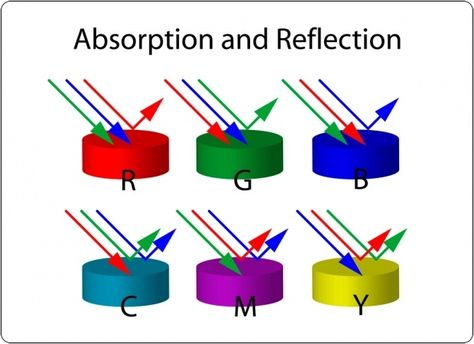
\includegraphics[width=\textwidth]{./figures/reflection.jpg}
      \end{center}

      % \begin{itemize}
      %   \setlength{\itemindent}{-0.7cm}
      % \item We observe outgoing light
      % \item Interested in object colour
      % \end{itemize}
    }
      \onslide*<4>{
      \begin{center}
        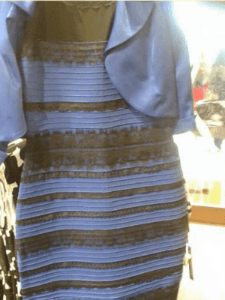
\includegraphics[height=3.5cm]{./figures/dress.png}
      \end{center}
      }

      \onslide*<5->{
      \begin{center}
        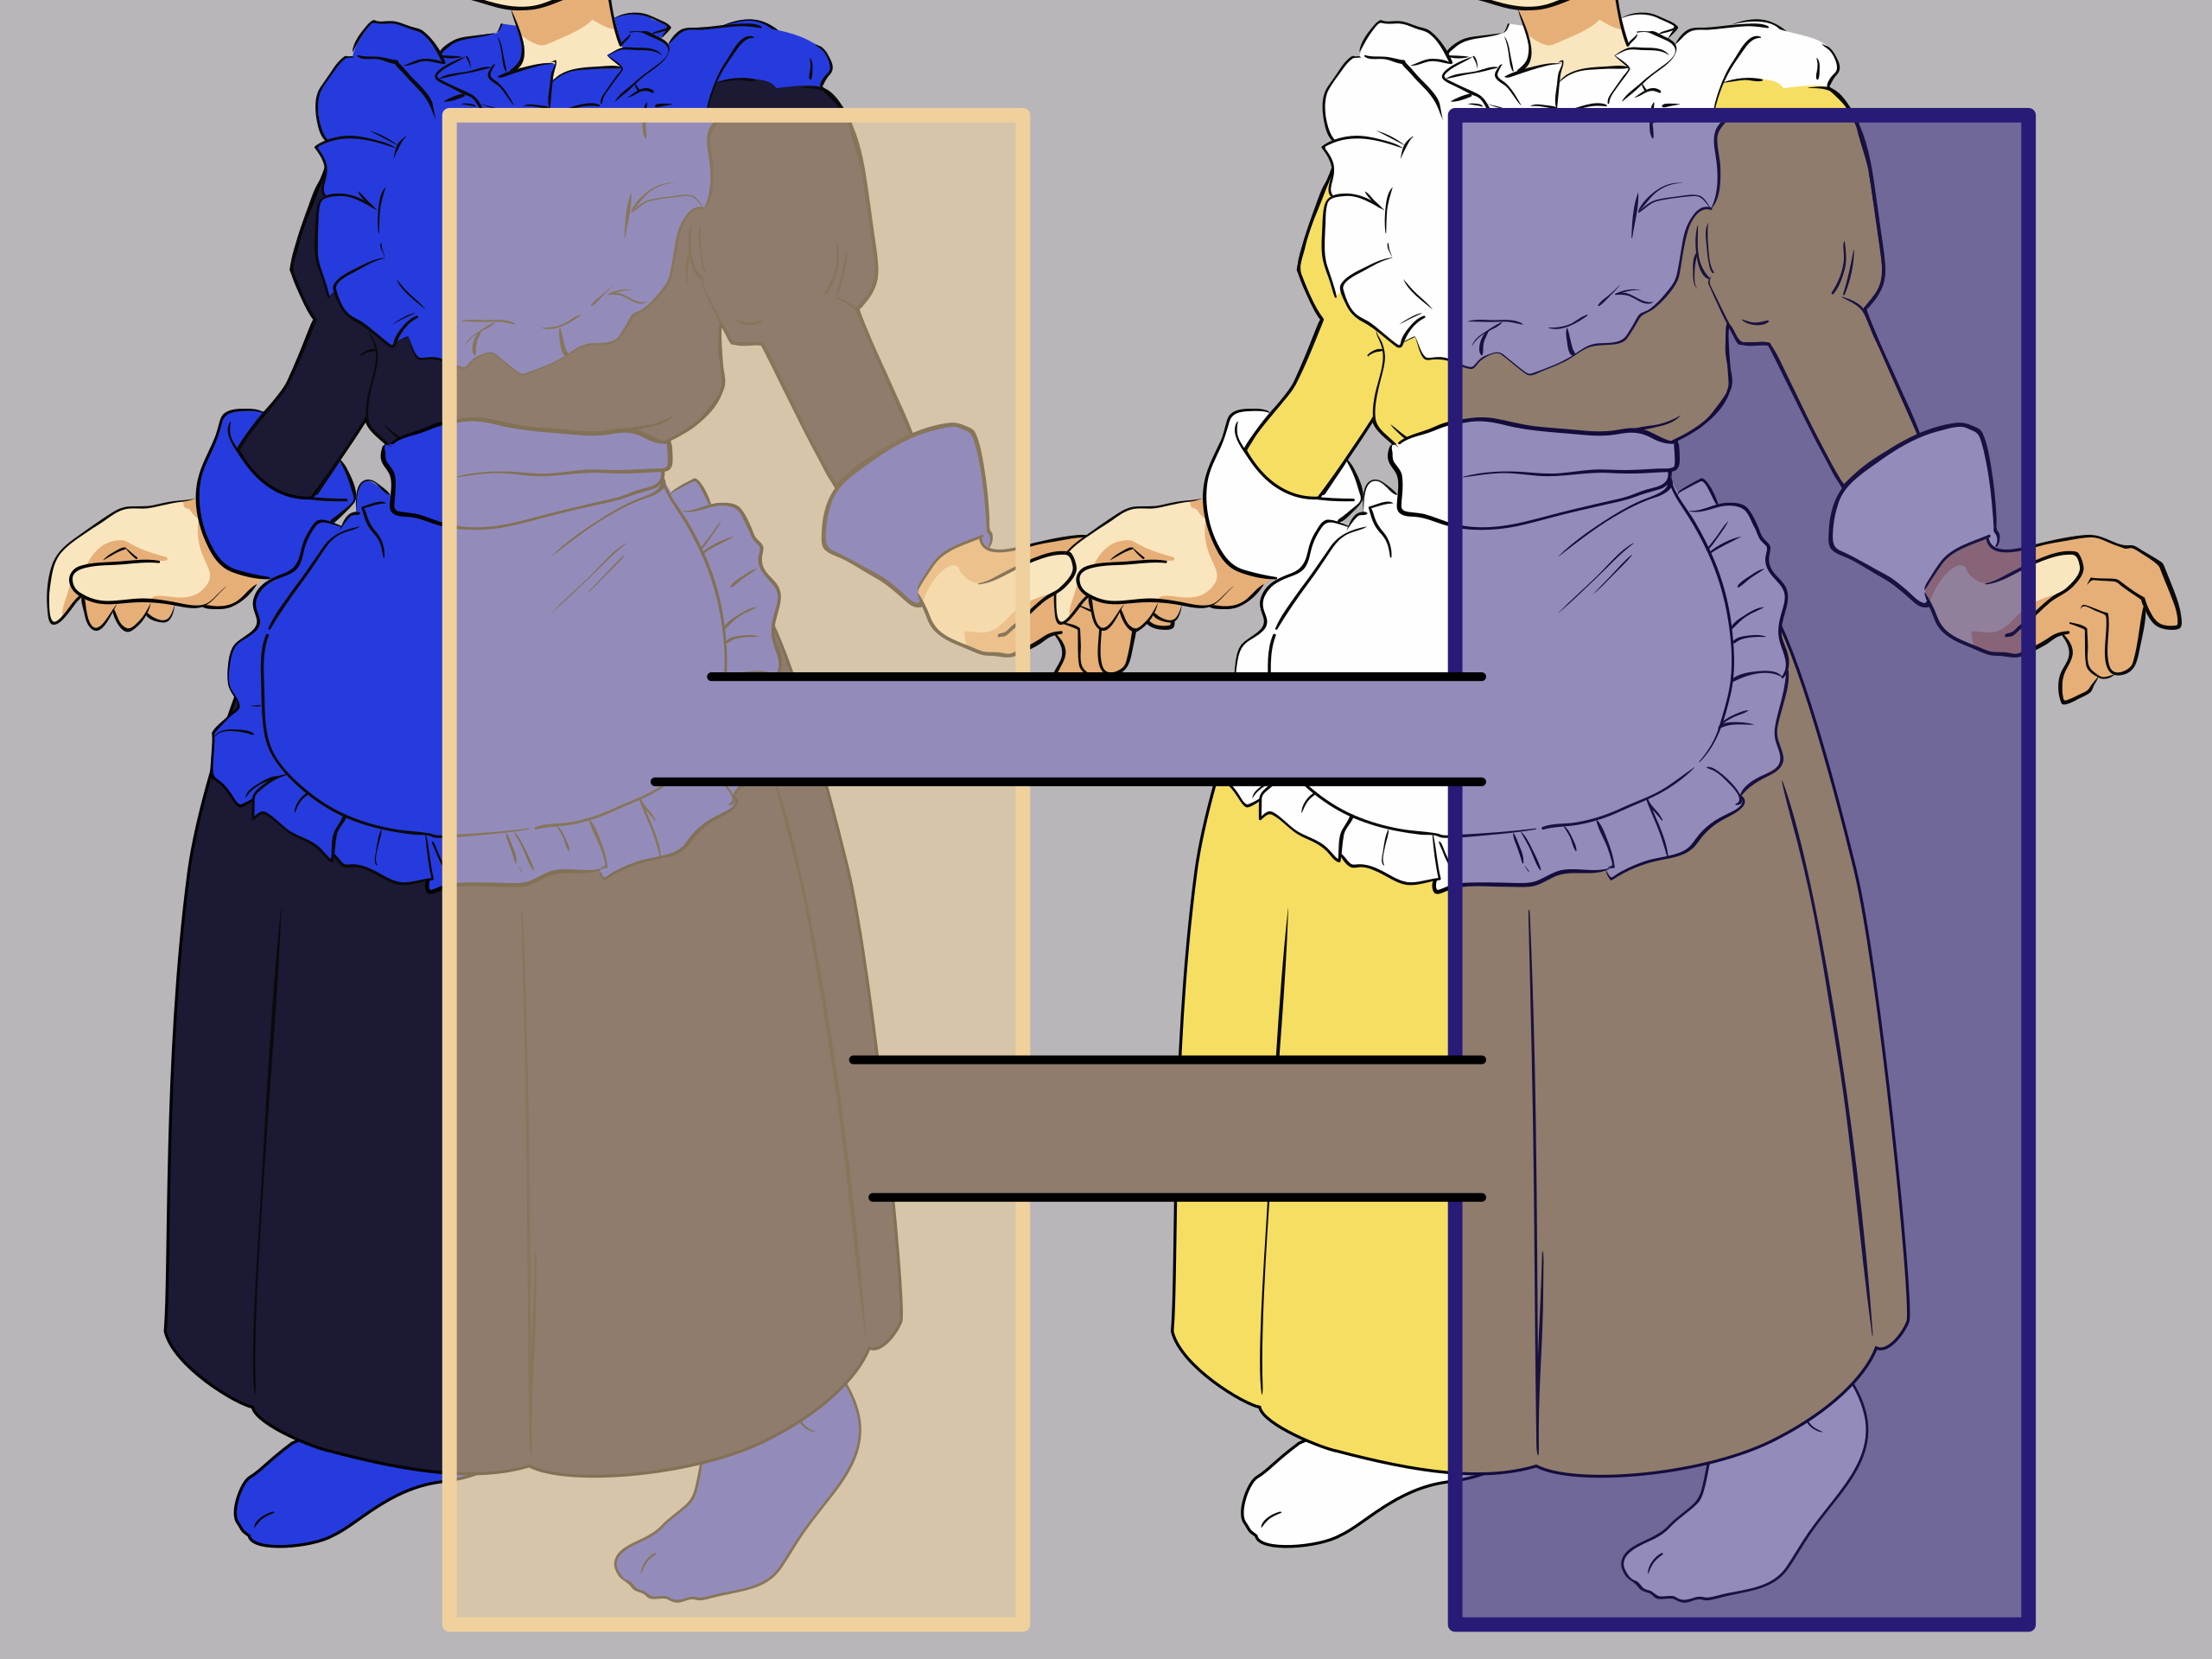
\includegraphics[height=3.5cm]{./figures/dress-explain.png}
      \end{center}
      }
      \end{overprint}
    \end{column}
    \hfill
  \end{columns}
  \onslide<6>{
\vspace{-0.6cm}

\begin{table}[]
\label{tab:blue}
\caption{\small{Left: $P(C|L=\ell,I)$, right: $P(C|L,\hyp_k)$ for $k\in\{1,2,3\}$.}}
\vspace{-0.2cm}
\begin{tabular}{lcc|ccc}
              & \textit{$I=\text{B}$} & $I=\text{Y}$ & $p_{B1} = 0.8$ & $p_{Y2} = 0.8$ & $p_{B3} = 0.5$ \\
$C=\text{WG}$ & \textit{$0.9$}        & $0.1$        & $0.74$               & $0.26$               & $0.5$                \\
$C=\text{BB}$ & $0.1$                 & $0.9$        & $0.26$               & $0.74$               & $0.5$               
\end{tabular}
\end{table}
}
\end{frame}

\begin{frame}{Representing uncertainty}
\begin{center}
{\Large White and Gold} or {\Large Blue and Black}?
\end{center} \pause

\begin{itemize}
\item Lighting situation was \textbf{ambiguous}, so prior determined posterior. \pause
\item Prior is subjective, but we can agree on reasoning! \pause
% \item Because of our \textbf{prior uncertainty} on the incoming light, we remain uncertain after observing data (\textbf{a posteriori}). \pause
\end{itemize}

So what could explain this phenomenon?\pause
\begin{itemize}
\item Our brains could have a biased prior, \pause
\item or the prior is 50-50, and we perceive our brain's best guess! \pause
% \item We \textbf{represent uncertainty} using a \textbf{probability distribution}. \pause
% \item Hence: \textbf{Probabilistic Inference} \pause
\end{itemize}

\begin{center}
        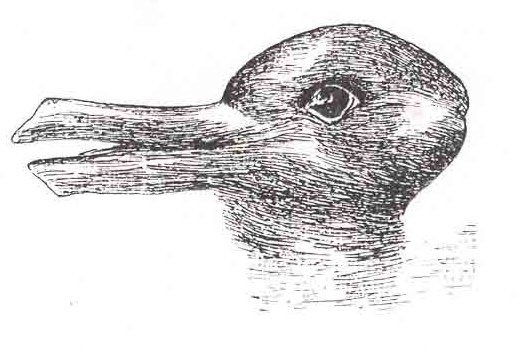
\includegraphics[height=2.7cm]{./figures/duck-rabbit.jpg}
\end{center} \pause
\vspace{-0.3cm}
\begin{itemize}
\item Guess: Our brain jumps to one interpretation, even if the belief is only mildly stronger. \pause
\item Wouldn't it be better if we kept track of all possibilities?
\end{itemize}
\end{frame}





\begin{frame}{Further Reading: Cox Axioms}
We discussed that probability can represent \emph{beliefs in statements}, and that in a certain way it extends propositional calculus to deal with uncertainty. \pause

\begin{itemize}
\item \citet{cox1946,cox1963} proposed \emph{axioms} that such a way of ``reasoning under uncertainty'' should satisfy.
\item Further claim: Probability theory is the \emph{only} way to reason under uncertainty!
\item This is controversial! Not everyone agrees to what degree this is proven, or which axioms are necessary.
\end{itemize} \pause

See e.g.~\citet{vanhorn2003cox}. \pause

\vspace{0.5cm}

Beware of looking into this! You end up doing philosophy, which is interesting, but not helpful to get things done...

\end{frame}


\begin{frame}{Further Reading: Dutch Books}
Map beliefs to bets: \\
 You take a bet if its expected value under your beliefs is positive.
\begin{itemize}
\item Example: For a coin for which you believe $P(\text{heads}) = p$, \\
where you get a payout of \emph{€1 if you win}, \\
you will pay up to \emph{€p to take the bet}.
\end{itemize} \pause

\vspace{0.3cm}

A Dutch book is a
\begin{itemize}
\item set of bets that you \emph{would take},
\item but that \emph{always leads you to lose money}!
\end{itemize} \pause

\vspace{0.3cm}

If you have \emph{inconsistent beliefs}, then you a Dutch book exists, e.g.:
\begin{itemize}
\item Belief $P(\text{heads}) = 0.9$ \textbf{and} $P(\text{tails}) = 0.9$ (inconsistent)
\item Bet 1: Pay €0.9 to bet on heads for a payout of €1.
\item Bet 2: Pay €0.9 to bet on tails for a payout of €1. \pause
\item Result: You always lose €0.8.
\end{itemize}

\vspace{0.3cm}\pause

Dutch book theorem: No Dutch book if you follow probability.
\end{frame}






% Flip-side of \textbf{uncertainty} is \textbf{belief}.

\begin{frame}{What is this course about?}
\pause
\begin{center}
\huge Inference
\end{center}
\pause
\begin{center}
{\large 
Given my \textbf{understanding} of how the world works} \pause \\
Given \textbf{incomplete information} about the world \pause \\
\Large \textbf{What do I know} about what I don't observe?
\end{center} \pause

\vspace{0.5cm}

\begin{itemize}[<+->]
\item Use probability to represent subjective state of \emph{uncertainty}.
\item Reduction in uncertainty is \emph{learning}!
\item Rules of probability describe learning \emph{process}.
\end{itemize}
\end{frame}


\begin{frame}{What is this course about?}

\vspace{0.5cm}

\begin{itemize}
  \item Specifying models by \emph{specifying beliefs} using probabilities. \pause
  \item \emph{Computing beliefs} about the world after seeing data. \pause
  \item Using uncertainty when making \emph{decisions}.
\end{itemize}

\vspace{0.5cm} \pause

The course will be mathematical! (but it's not a maths course)
\begin{itemize}
\item We will discuss proofs (although focussing on the big picture).
\item We will analyse the behaviour of algorithms.
\item Exam will require you to demonstrate ability to apply mathematical principles.
\item BUT, hopefully you gain an intuition into the principles too.
\end{itemize}
\end{frame}



% \begin{frame}{Exercises}
% To get warmed up, I recommend doing a few exercises.
% \end{frame}





\begin{frame}{Course outline}
\begin{enumerate}[I)]
\item Bayesian brainteasers (graphical models, tractable inference) \\
How do we put problems into the mathematical formalism? What is a model? How do we formulate assumptions in models?
\vspace{0.5cm}
\item Gaussian processes \\
Specifying models, computing beliefs.
\vspace{0.5cm}
\item Decision Theory \& Bayesian optimisation \\
Using uncertainty to take actions.
\vspace{0.5cm}
\item Approximate inference \\
What happens if we cannot compute our beliefs exactly?
\vspace{0.5cm}
\item Modern applications, e.g.~generative models \\
How is this used right now?
\end{enumerate}
\end{frame}


\begin{frame}{Why take this course?}
Develop toolset of:
\begin{itemize}
\item (Bayesian) statistical methods\footnote{There is more to statistics than this course!} \pause \\
Useful to solve problems (next slide)
\item Dealing with distributions in deep learning \pause \\
Generative modelling (e.g.~VAEs, diffusion models) \pause
\end{itemize}

\vspace{0.3cm}

Develop understanding of: \pause
\begin{itemize}
\item Reasoning under uncertainty and ambiguity \pause \\
(Arguably): All good procedures must map onto Bayesian inference somehow \pause
\item The underlying process of what deep learning needs to solve \pause \\
Combining cues from disparate sources
\end{itemize}
\end{frame}


\begin{frame}{Why take this course?}
% \begin{itemize}
% \item Probably not necessary if you want to focus only on implementing methods. \pause
% \item Very helpful if you want to \emph{understand} methods, \pause \\
% ... or develop \emph{new} methods. \pause
% \end{itemize}

I would recommend if you want to do
\begin{itemize}
\item data science, i.e.~building models for careful prediction,
\item development of new machine learning models / techniques,
\item machine learning research.
\end{itemize} \pause

\vspace{0.5cm}
Probably not necessary if you want to focus on implementing ML models, or ML infrastructure.
\end{frame}


\begin{frame}{What problems can we solve?}
  \begin{itemize}
    \item Low data prediction (how (un)certain am I?)
    \item Experiment design (what data should I gather next?)
    \item Data fusion (How should I combine information sources?)
    \item Learning (How should my belief change to match the world?)
    \item Decision making (Should I take a risk or play it safe?)
  \end{itemize}
\end{frame}


\begin{frame}{Prerequisites}

\begin{itemize}
  \item Good understanding of Mathematics for Machine Learning, e.g.:
  \begin{itemize}
  \item Linear algebra (eigendecompositions etc)
  \item Probability and basic statistics
  \item Vector calculus
  \item Gradient-based optimisation
  \end{itemize}
  \item Python coding
\end{itemize}
\begin{center}
  \url{https://mml-book.com}
\end{center}
\end{frame}




\begin{frame}{Expectations}

What is expected for the exam:
\begin{itemize}
  \item Knowledge of topics discussed
  \item Awareness of why topics are relevant
  \item Derive methods using mathematical concepts discussed
  \item Analyse methods using mathematical concepts discussed
\end{itemize}

\vspace{0.5cm}


How to study \& revise:
\begin{itemize}
\item Join the lectures in person, engage, share your questions
\item Think about how how theory applies in different settings
\item Do the exercises
\end{itemize}


\end{frame}




\begin{frame}{Highly Recommended Reading}
Information Theory, Inference, and Learning Algorithms \citep{itila}
\begin{itemize}
\item \S2.1 (4pgs): Refresher of probability + notation we will use.
\item \S2.2 (1pg): Probability as belief.
\item \S2.3 (5pgs): Examples of Bayes rule. Exercises + solutions are very illustrative.
\end{itemize}

\emph{You really should read this.}

\vspace{0.5cm}
See EdStem for links to books. 
\end{frame}



\begin{frame}{Practicalities}
\begin{itemize}
\item Two assessed coursework (on Part II \& III and IV).
\begin{itemize}
\item Coding exercises assessed by unittests, designed to \emph{teach}.
\item Exam is designed to \emph{assess}.
\end{itemize} \pause
\item Q\&A sessions most Fridays: Quickest way to get an answer to your question. \pause
\item Feedback: TAs+I are happy to give feedback on your solutions to exercises (e.g.~if you want to know if you did enough steps) \\
Friday Q\&A session or on EdStem. \pause
\item I would like 
\item I will look at EdStem questions once per week.
\end{itemize}
\end{frame}



\begin{frame}{Questions?}
Hopefully this gives you an overview of the course.

\vspace{0.5cm}

\begin{center}
\Huge \emph{Questions?}
\end{center}
\end{frame}




\begin{frame}[t,allowframebreaks]
\frametitle{References}
\linespread{1.0}
\tiny
% \bibliographystyle{abbrv}
\bibliographystyle{apalike}
\bibliography{../includes/pi-literature.bib}
\end{frame}





















\end{document}
%%% Local Variables: 
%%% mode: latex
%%% TeX-master: t
%%% End: 
